
\documentclass[12pt]{article}
\usepackage[english]{babel}
\usepackage[T1]{fontenc}
\usepackage[utf8]{inputenc}
\usepackage{delarray,amsmath,bbm,epsfig,slashed}
\newcommand{\pat}{\partial}
\newcommand{\be}{\begin{equation}}
\newcommand{\ee}{\end{equation}}
\newcommand{\bea}{\begin{eqnarray}}
\newcommand{\eea}{\end{eqnarray}}
\newcommand{\abf}{{\bf a}}
\newcommand{\Zmath}{\mathbf{Z}}
\newcommand{\Zcal}{{\cal Z}_{12}}
\newcommand{\zcal}{z_{12}}
\newcommand{\Acal}{{\cal A}}
\newcommand{\Fcal}{{\cal F}}
\newcommand{\Ucal}{{\cal U}}
\newcommand{\Vcal}{{\cal V}}
\newcommand{\Ocal}{{\cal O}}
\newcommand{\Rcal}{{\cal R}}
\newcommand{\Scal}{{\cal S}}
\newcommand{\Lcal}{{\cal L}}
\newcommand{\Hcal}{{\cal H}}
\newcommand{\hsf}{{\sf h}}
\newcommand{\half}{\frac{1}{2}}
\newcommand{\Xbar}{\bar{X}}
\newcommand{\xibar}{\bar{\xi }}
\newcommand{\barh}{\bar{h}}
\newcommand{\Ubar}{\bar{\cal U}}
\newcommand{\Vbar}{\bar{\cal V}}
\newcommand{\Fbar}{\bar{F}}
\newcommand{\zbar}{\bar{z}}
\newcommand{\wbar}{\bar{w}}
\newcommand{\zbarhat}{\hat{\bar{z}}}
\newcommand{\wbarhat}{\hat{\bar{w}}}
\newcommand{\wbartilde}{\tilde{\bar{w}}}
\newcommand{\barone}{\bar{1}}
\newcommand{\bartwo}{\bar{2}}
\newcommand{\nbyn}{N \times N}
\newcommand{\repres}{\leftrightarrow}
\newcommand{\Tr}{{\rm Tr}}
\newcommand{\tr}{{\rm tr}}
\newcommand{\ninfty}{N \rightarrow \infty}
\newcommand{\unitk}{{\bf 1}_k}
\newcommand{\unitm}{{\bf 1}}
\newcommand{\zerom}{{\bf 0}}
\newcommand{\unittwo}{{\bf 1}_2}
\newcommand{\holo}{{\cal U}}
%\newcommand{\bra}{\langle}
%\newcommand{\ket}{\rangle}
\newcommand{\muhat}{\hat{\mu}}
\newcommand{\nuhat}{\hat{\nu}}
\newcommand{\rhat}{\hat{r}}
\newcommand{\phat}{\hat{\phi}}
\newcommand{\that}{\hat{t}}
\newcommand{\shat}{\hat{s}}
\newcommand{\zhat}{\hat{z}}
\newcommand{\what}{\hat{w}}
\newcommand{\sgamma}{\sqrt{\gamma}}
\newcommand{\bfE}{{\bf E}}
\newcommand{\bfB}{{\bf B}}
\newcommand{\bfM}{{\bf M}}
\newcommand{\cl} {\cal l}
\newcommand{\ctilde}{\tilde{\chi}}
\newcommand{\ttilde}{\tilde{t}}
\newcommand{\ptilde}{\tilde{\phi}}
\newcommand{\utilde}{\tilde{u}}
\newcommand{\vtilde}{\tilde{v}}
\newcommand{\wtilde}{\tilde{w}}
\newcommand{\ztilde}{\tilde{z}}

% David Weir's macros


\newcommand{\nn}{\nonumber}
\newcommand{\com}[2]{\left[{#1},{#2}\right]}
\newcommand{\mrm}[1] {{\mathrm{#1}}}
\newcommand{\mbf}[1] {{\mathbf{#1}}}
\newcommand{\ave}[1]{\left\langle{#1}\right\rangle}
\newcommand{\halft}{{\textstyle \frac{1}{2}}}
\newcommand{\ie}{{\it i.e.\ }}
\newcommand{\eg}{{\it e.g.\ }}
\newcommand{\cf}{{\it cf.\ }}
\newcommand{\etal}{{\it et al.}}
\newcommand{\ket}[1]{\vert{#1}\rangle}
\newcommand{\bra}[1]{\langle{#1}\vert}
\newcommand{\bs}[1]{\boldsymbol{#1}}
\newcommand{\xv}{{\bs{x}}}
\newcommand{\yv}{{\bs{y}}}
\newcommand{\pv}{{\bs{p}}}
\newcommand{\kv}{{\bs{k}}}
\newcommand{\qv}{{\bs{q}}}
\newcommand{\bv}{{\bs{b}}}
\newcommand{\ev}{{\bs{e}}}
\newcommand{\gv}{\bs{\gamma}}
\newcommand{\lv}{{\bs{\ell}}}
\newcommand{\nabv}{{\bs{\nabla}}}
\newcommand{\sigv}{{\bs{\sigma}}}
\newcommand{\notvec}{\bs{0}_\perp}
\newcommand{\inv}[1]{\frac{1}{#1}}
%\newcommand{\xv}{{\bs{x}}}
%\newcommand{\yv}{{\bs{y}}}
\newcommand{\Av}{\bs{A}}
%\newcommand{\lv}{{\bs{\ell}}}

%\newcommand\bsigma{\vec{\sigma}}
\hoffset 0.5cm
\voffset -0.4cm
\evensidemargin -0.2in
\oddsidemargin -0.2in
\topmargin -0.2in
\textwidth 6.3in
\textheight 8.4in

\begin{document}

\normalsize

\baselineskip 14pt

\begin{center}
{\Large {\bf Open Quantum Systems \ \  Answers to Exercise Set 2 \& 3 - JPBK }}\\
{\large { Jake Muff}}\\
jake.muff@helsinki.fi \\
{Student number: 015361763}\\
{10/10/2020}
\end{center}


\section{Answers}
\begin{enumerate}

\item Problem 2.1. Obtain heat in a nearly quasi-static drive in a two level system.
%Question 1 Answer here
\\
This question troubled me, in particular, the meaning behind "nearly quasi-static". I'm not sure what this means as a quasi-static process is one in which it is almost or nearly static or stationary so the term "nearly" here doesn't seem to have any meaning. 
I read the paper \cite{4}, mentioning quasistatic drive and I will assume that you wish us to study the Quasistatic limit in which $W$ is close to the ideal limit of $-K_B T ln(2)$ or the case where there is equality $W = Q$ 
\\
\\
There is also the case from where the Hamiltonian simply reads  \cite{10}
$$ H = E_C (n-n_g )^2 $$
For a single electron box where $E_C = \frac{e^2}{2C}$. The cited paper mentions 'sweeping' out the quasi-static drive to $n_g = 1/2$ allowing for the increase in the entropy of the charge system giving 
$$ \Delta S = K_B ln(2) $$ 
And due to the process being quasi-static, $\Delta S$ is equal to the increase in the entropy of the bath so
$$ \Delta Q = T \Delta S = K_B T ln(2) $$ 
Maxwell's demon allows the system to be a "nearly" quasistatic driven system as the degeneracy can be 'ramped', turning the process cyclic and extracting heat of $K_B T ln(2) $ from the bath. Experimentally, Jukka finds that the average heat dissapated is 
$$ Q_{avg} = -0.75 K_B T ln(2) $$ 

%On the other hand, not taking into account the lecture notes or supplementary material I considered a standard two-level system between a small open system and a heat reservoir in which the energy of the system can be related to the first law of thermodyanmics 


\item Problem 2.2: Proof of Landauer's Principle
\\
Consider a two level system with thermodynamic entropy $K_B ln(2)$, which was proven by Von Neumann in 1949. The process of the erasure of the bit gives us a starting point of a microstate where the entropy is zero. \\
According to the 2nd law of thermodynamics, entropy cannot decrease - it must go somewhere-, so it is 'transferred' to the environment with temperature $T$ giving us an energy cost of atleast $K_B T ln(2)$ so 
$$ E \geq K_B T ln(2) $$
This is a very simple version where the proof as laid out by Von Neumann was not explicitely stated. Thermodynamic entropy cannot be so easily related to the information entropy. 
Jukka Pekola wrote a very interesting paper [3] which related the reversal to Maxwell's limit of thermodynamic efficiency and shows that it is consistent with the 2nd law of thermodynamics. 
\\
A more rigourous mathematical proof is the following: 
\\
The work extracted during isothermal quasistatic expansion is given by 
$$ \Delta Q = \Delta W = \int_{\frac{V}{2}}^V \rho dV $$
$$ = \int_{\frac{V}{2}}^V \frac{K_B T}{V} dV $$ 
$$ = K_B T ln(2) $$ 
The second law of thermodyanmics states that the entropy of an isolated system can never decrease with time. Applying this to the above fixes $\Delta Q$ 
$$ \Delta Q \geq K_B T ln(2) $$
$$ E \geq K_B T ln(2) $$
This can also be proven from isothermal compression as well 
$$ \Delta Q = - \Delta W $$ 
$$ = - \int_{v}^{\frac{V}{2}} \rho dV = - \int_{V}^{\frac{V}{2}} \frac{K_B T}{V} dV $$
$$ = K_b T ln(2) $$




\item Problem 3.1.
\begin{enumerate}
    \item Why CBT in the universal regime where $ E_C << K_B T $ can be considered a primary thermometer? 
    \\
    In a 'Primary' thermometer the measuredd property of matter is known so well that temperature can be calculated without any unknown quantities. Which is CBT we have 
    $$ \frac{G}{G_T} = 1 - \frac{2E_C}{K_B T} g \big( \frac{eV}{2K_B T}\Big) $$ 
    $$ g(x) = \frac{x sinh(x) - 4sinh^2 (x/2)}{8sinh^4 (x/2)} $$
    So 
    $$ \frac{G}{G_T} = 1 - \frac{e^2/C}{K_B T} \frac{ xsinh(x) - 4sinh^2 (x/2)}{8sinh^4 (x/2)} $$
    Where 
    $$ x = \frac{eV}{2 K_B T} $$
    And for $N=2$ case 
    $$ E_C = \frac{e^2}{2C} $$ 
    In the case where $E_C << K_B T$ the normalized conductance does not depend on the CBT's dimensions and can be considered a primary thermometer (As $2E_c / K_B T \rightarrow 0$)
    \item If we consider the full width half minimum of the normalized conductance so $V = V_{1/2}$ and set this to $\lambda$ 
    $$ \frac{eV_{1/2}}{N K_B T} = \lambda $$
    $$ V_{1/2} = \frac{\lambda N K_B T}{e}$$
    The numerical number was calculated to be 
    $$ \lambda = 5.434 $$ 
    
    \begin{figure}[h]
        \centering
        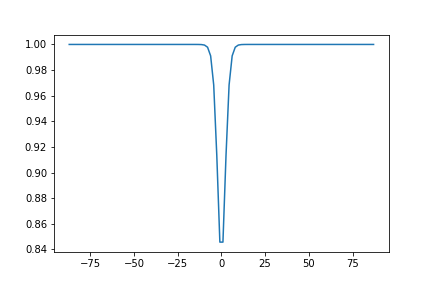
\includegraphics[width=10cm]{plot.png}
        \caption{Plot of the normalized conductance using matplotlib. Axis values aren't quite correct but this shows an inverse bell curve. A full width half minimum approach can be used to calcuate $V_{1/2}$}
        \end{figure}
\end{enumerate}



\end{enumerate}

\section{Note}
I found these exercises particularly hard, mainly due to the nature of the questions, however I believe this was due to getting use to the particular thermodynamic jargon used of which I am not used to. I found an abundance of papers and research completed online (mostly by Jukka Pekola) which taught me a great deal and helped supplement what was taught in the lectures, however did not help me to complete the questions theoretically. I have attached references in my bibliography at the bottom to works which I heavily relied on. 

\begin{thebibliography}{9}
    \bibitem{1}
    Anna Feshchenko. \\
    \textit{Electron Themometry, refrigeration and heat transport in nanostructures at sub-kelvin temperatures}
    Doctoral Thesis, Department of Applied Physics, Low Temperature Laboratory, Aalto University
    \bibitem{2}
    M. Tinkham 
    Introduction to Superconductivity
    Dover Publications, 2004
    \bibitem{3}
    Averin, Dmitri V. and Pekola, Jukka P. \\
    \textit{Reversing the Landauer’s erasure: Single-electron Maxwell’s demon operating at the limit of thermodynamic efficiency}.
    Jan 2017. 
    \bibitem{4}
    Jonne V. Koskia, Ville F. Maisia, Jukka P. Pekola, and Dmitri V. Averind.
    \textit{Experimental realization of a Szilard engine with
    a single electron}.
    August 2014. 
    \bibitem{5}
    J. V. Koski, V. F. Maisi , T. Sagawa and J. P. Pekola. 
    \textit{Experimental study of mutual information in a Maxwell Demon}. 
    May 2014. 
    \bibitem{6}
    Gavin E. Crooks.
    \textit{Nonequilibrium Measurements of Free Energy
    Differences for Microscopically Reversible
    Markovian Systems}.
    October 1997. 
    \bibitem{7}
    Rogério J. de Assis, José S. Sales, Udson C. Mendes, and Norton G. de Almeida.
    \textit{Two-level quantum Otto heat engine operating with unit efficiency far from the quasi-static
    regime under a squeezed reservoir}.
    March 2020.
    \bibitem{8}
    Enrique Muñoz, Francisco J. Peña and Alejandro González.
    \textit{Magnetically-Driven Quantum Heat Engines:
    The Quasi-Static Limit of Their Efficiency}
    May 2016. 
    \bibitem{9}
    Robert Alicki.
    \textit{Introduction to Quantum Thermodynamics:
    History and Prospects}
    May 2018.
    \bibitem{10} 
    Vasco Cavina Andrea Mari and Vittorio Giovannetti.
    \textit{Slow dynamics and thermodynamics of open quantum systems}
    August 2017. 
    \bibitem{11}
    Pekola, Jukka P
    \textit{Towards quantum thermodynamics in electronic circuits}.
    2015.

\end{thebibliography}
\end{document}

